%%%%%%%%%%%%%%%%%%%%%%%%%%%%%%%%%%%%%%%%%%%%%%%%%%%%%%%%%%%%%%%%%%% 
%                                                                 %
%                            CHAPTER                              %
%                                                                 %
%%%%%%%%%%%%%%%%%%%%%%%%%%%%%%%%%%%%%%%%%%%%%%%%%%%%%%%%%%%%%%%%%%% 

\chapter{Accelerating the software implementation using HLS}
\label{ch:HardwareImpl}

\section{Analysing software performance}
\label{swAnalyse}

In the SDSoC environment, it is possible to analyze the software running on the SoC chip using a TCF profiler. After running this analysis, the TCF profiler returns an overview of the functions, sorted on the amount of time spent when running. The analysis is shown in figure~\ref{fig:softwareFunctionUsage}

\begin{figure}[H]
	\centering
	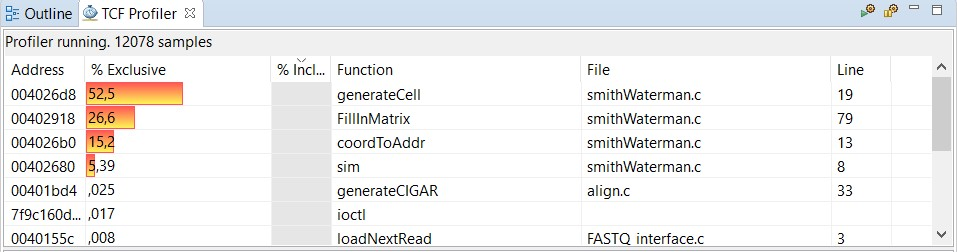
\includegraphics[width=0.75\textwidth]{speedup/softwareFunctionUsage.jpg}
	\caption{a TCF profile of the software implementation}
	\label{fig:softwareFunctionUsage}
\end{figure}

When examining this analysis, we should keep in mind that the generateCell, coordToAddr, and sim functions are inline functions used in the FillInMatrix method. Just as suspected the software spends almost all of its time in these methods, so it's worth trying to accelerate these functions.

\section{Recoding parts of the software to be more hardware friendly}

\subsection{Recoding the Cell generation layer}

In 2011, Vermij E. (Delft University of Technology, The Netherlands) studied RVE (recursive variable expansion)~\cite{Vermij}. He discusses the most efficient ways to program a processing element to generate one value in the alignment matrix. His results can be found in figure~\ref{fig:PE}. 

\begin{figure}[H]
	%src=file:///D:/Erasmus/thesis/interessante%20papers/masterthesis%20Smith-Waterman%20op%20FPGA%20(TU%20Delft).pdf
	\centering
	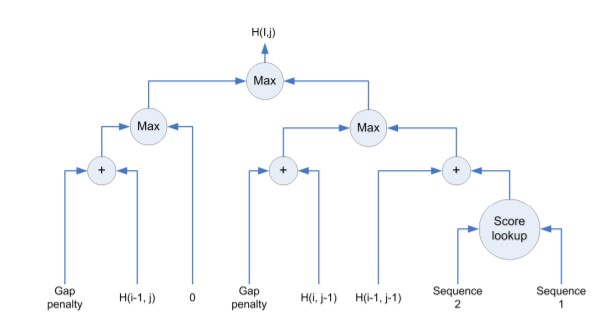
\includegraphics[width=0.75\textwidth]{speedup/PE.jpg}
	\caption{The optimal processing found by Vermij E.~\cite{Vermij}}
	\label{fig:PE}
\end{figure}

It seemed like a good idea to reimplement the generatecell function, using this newly found scheme. However, it is also important to keep track of where the value comes from. Therefore, the following (new) code was adopted for generating a CELL:

\begin{lcverbatim}
//calculate the possible  values
CELL diagonalCELL = { diagonal.value + sim(refVal, seqVal), 1 };
CELL leftCELL = { left.value - gp, 2 };
CELL upCELL = { up.value - gp, 3 };
CELL zeroCELL = { 0, 0 };

CELL upstreamA = (leftCELL.value > upCELL.value) ? leftCELL : upCELL;
CELL upstreamB = (diagonalCELL.value > zeroCELL.value) ? 
diagonalCELL : zeroCELL;

CELL newCell = (upstreamA.value > upstreamB.value) ? upstreamA : upstreamB;

//Return the cell:
return newCell;
\end{lcverbatim}
Where the second attribute in the CELL type is the direction.

\subsection{Recoding the FillIn layer}

HLS does not support input and output from the same memory locations in hardware. Therefore, the Fillin layer also has to be recoded. We will take a look at the data dependencies again:

\begin{figure}[H]
	\centering
	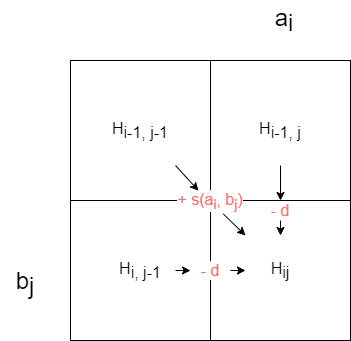
\includegraphics[width=0.3\textwidth]{ExisMethods/Dependencies_SW.png}
	\caption{Data dependencies for generating a cell in the alignment matrix}
	\label{fig:DatDep2}
\end{figure}

Since the current cell only depends on the left-up 3 cells, we can compute every cell on the diagonal in parallel. Therefore, 3 arrays where created: one contains the current diagonal being generated, one contains the previous diagonal for the cell above and the cell to the left of the current generated cell, and one for the diagonal before that. This last array will house the left-up cell also needed for the new cell generation. A schematic of the data structures used can be found in table~\ref{tbl:arraytable}

\begin{table}[H]
	\centering
	\begin{tabular}{|l|lllllllllll|l|l|l|}
		\cline{1-10} \cline{13-15}
		\multicolumn{1}{|c|}{\textbf{}} & \multicolumn{1}{r|}{\textbf{ref}} & \multicolumn{1}{l|}{\textbf{T}} & \multicolumn{1}{l|}{\textbf{G}} & \multicolumn{1}{l|}{\textbf{T}} & \multicolumn{1}{l|}{\textbf{T}} & \multicolumn{1}{l|}{\textbf{A}} & \multicolumn{1}{l|}{\textbf{C}} & \multicolumn{1}{l|}{\textbf{G}} & \multicolumn{1}{l|}{\textbf{G}} & \textbf{}       & \textbf{} & \textbf{ppD}              & \textbf{pD}               & \textbf{cD}               \\ \cline{1-10} \cline{13-15} 
		\textbf{seq}                    & 0                                 & 0                               & 0                               & 0                               & 0                               & \cellcolor[HTML]{9AFF99}0       & \cellcolor[HTML]{96FFFB}0       & \cellcolor[HTML]{FFCCC9}0       & 0                               &                 &           & \cellcolor[HTML]{9AFF99}0 & \cellcolor[HTML]{96FFFB}0 & \cellcolor[HTML]{FFCCC9}0 \\ \cline{1-1} \cline{13-15} 
		\textbf{G}                      & 0                                 & 0                               & 3                               & 1                               & \cellcolor[HTML]{9AFF99}0       & \cellcolor[HTML]{96FFFB}0       & \cellcolor[HTML]{FFCCC9}?       &                                 &                                 &                 &           & \cellcolor[HTML]{9AFF99}0 & \cellcolor[HTML]{96FFFB}0 & \cellcolor[HTML]{FFCCC9}? \\ \cline{1-1} \cline{13-15} 
		\textbf{G}                      & 0                                 & 0                               & 3                               & \cellcolor[HTML]{9AFF99}1       & \cellcolor[HTML]{96FFFB}0       & \cellcolor[HTML]{FFCCC9}?       &                                 &                                 &                                 & =\textgreater{} &           & \cellcolor[HTML]{9AFF99}1 & \cellcolor[HTML]{96FFFB}0 & \cellcolor[HTML]{FFCCC9}? \\ \cline{1-1} \cline{13-15} 
		\textbf{T}                      & 0                                 & 3                               & \cellcolor[HTML]{9AFF99}1       & \cellcolor[HTML]{96FFFB}6       & \cellcolor[HTML]{FFCCC9}?       &                                 &                                 &                                 &                                 &                 &           & \cellcolor[HTML]{9AFF99}1 & \cellcolor[HTML]{96FFFB}6 & \cellcolor[HTML]{FFCCC9}? \\ \cline{1-1} \cline{13-15} 
		\textbf{T}                      & 0                                 & \cellcolor[HTML]{9AFF99}3       & \cellcolor[HTML]{96FFFB}1       & \cellcolor[HTML]{FFCCC9}?       &                                 &                                 &                                 &                                 &                                 &                 &           & \cellcolor[HTML]{9AFF99}3 & \cellcolor[HTML]{96FFFB}1 & \cellcolor[HTML]{FFCCC9}? \\ \cline{1-1} \cline{13-15} 
		\textbf{G}                      & \cellcolor[HTML]{9AFF99}0         & \cellcolor[HTML]{96FFFB}1       & \cellcolor[HTML]{FFCCC9}?       &                                 &                                 &                                 &                                 &                                 &                                 &                 &           & \cellcolor[HTML]{9AFF99}0 & \cellcolor[HTML]{96FFFB}1 & \cellcolor[HTML]{FFCCC9}? \\ \cline{1-1} \cline{13-15} 
	\end{tabular}
	\caption{The 3 newly created arrays to house the data needed for generating the next diagonal of cells. The '?' in the cD array (red) represents cells currently being generated. Notice that all the information needed to generate the new cell is present in the other 2 arrays}
	\label{tbl:arraytable}
\end{table}

Also, keep note that the FillIn layer should keep track of the maximum location in the matrix. Having gained this new information, we can recode the FillInlayer as follows:

\begin{enumerate}
	\item Create the arrays $ppD$, $pD$ and $cD$. They should be the length of the sequence. All are initialized on zeros.
	\item Start the current diagonal at the second column.
	\item \label{everyCell}For every cell at the diagonal, do the following:
	\begin{enumerate}
		\item Check for edge cases. The row has to be smaller than the length of the sequence, the column can't be 0 or smaller and the column can't be bigger than the length of the reference.
		\item Generate the new cell using the data in the $ppD$ and $pD$ arrays.
		\item Write this new cell to memory, and its value to the cD array.
		\item Check if it is bigger than the current maximum. If so, the current maximum should be this new cell. 
	\end{enumerate}
	\item Set current diagonal to the next one.
	\item Shift the values ($cD \rightarrow pD$ and $pD \rightarrow ppD$) and repeat from step~\ref{everyCell}, until the total matrix is filled.
	\item Return the position of the maximum to the alignment level.
\end{enumerate}

Note that by programming the Fill in Layer this way, there is no need to read cells from memory, since they can be generated using the arrays. Only the reference and read sequences should be read from memory. 

\section{Hardware acceleration}

When accelerating the application, it was decided to implement the FillIn and cell generation layer in hardware, since they are the functions where most computational time is spent (see Section~\ref{swAnalyse}). Therefore, they were merged into 1 convenient function, which will be transferred to the programmable hardware. 

\subsection{DMA}

DMA or \text{Direct Memory Access} allows certain hardware systems in the computer to access the main system memory independent of the CPU. This can be of importance to the performance since the hardware system requires a lot of data movement between to and from the memory. The arrays (ref, seq, and matrix) are available in the memory, which means the programmable hardware should be able to access these arrays using DMA. 

\begin{figure}[H]
	\centering
	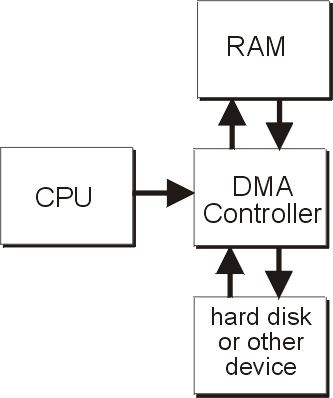
\includegraphics[width=0.25\textwidth]{speedup/dma.png}
	\caption{Schematic of a system using DMA}
	\label{fig:DMA}
\end{figure}

The following pragmas were used for the DMA:
\begin{lcverbatim}
#pragma SDS data access_pattern(ref:SEQUENTIAL, seq:SEQUENTIAL, 
	matrix:SEQUENTIAL)
#pragma SDS data sys_port(ref:AFI, seq:AFI, matrix:AFI)
#pragma SDS data mem_attribute(ref:PHYSICAL_CONTIGUOUS, 
	seq:PHYSICAL_CONTIGUOUS, matrix:PHYSICAL_CONTIGUOUS)
#pragma SDS data zero_copy(ref[0:refMax], seq[0:seqMax], 
	matrix[0:refMax*seqMax])
\end{lcverbatim}
\begin{itemize}
	\item \textbf{access\_pattern} can be either SEQUENTIAL or RANDOM. It specifies the data access pattern by the hardware to the memory. If SEQUENTIAL is used, the interface will be a stream (e.g. ap\_fifo). On the other hand, when RANDOM is used, a RAM interface will be generated.
	\item \textbf{sys\_port} can be ACP, AFI, GP or MIG. It specifies on which level the memory is interfaces. 
	\begin{itemize}
		\item ACP: Allows hardware functions to have cache-coherent access to DDR using the PS L2 cache.
		\item AFI: Hardware functions have fast non-cache coherent access to DDR via the PS memory controller.
		\item GP: The processor directly writes/reads data to/from hardware function. This would be inefficient for large data transfers.
		\item MIG: Hardware functions access DDR from PL via a MIG IP memory controller.
	\end{itemize}
	We have quite a large amount of data, so GP doesn't seem like a good option. Likewise, the memory will be accessed uniform, we have no use for a cache as this would just slow it down. Therefore the AFI was selected.
	\item \textbf{mem\_attribute} can be either PHYSICAL\_CONTIGUOUS or NON\_PHYSICAL\_CONTIGUOUS. The default value is NON\_PHYSICAL\_CONTIGUOUS. PHYSICAL\_CONTIGUOUS is used for memory allocated with sds\_alloc. Likewise, NON\_PHYSICAL\_CONTIGUOUS is used with memory allocated using malloc.
	\item \textbf{zero\_copy} means that the hardware function accesses the data directly from shared memory through an AXI master bus interface.
\end{itemize}

\paragraph{The data\_pack pragma} The data\_pack pragma is used on the matrix since it is an array of structs (CELL type). This packs the data fields of a struct into a single scalar. The bitwidth of the packed struct is the sum of its attributes.

The bitwidth of (packed) data on the AXI but must be a power of 2, to interface with the memory. Therefore, it was chosen to change the CELL\_VALUE type to an int16\_t and the direction to uint16\_t. This is however quite wasteful towards memory usage. It can be optimized by remodeling some of the code, but due to time constraints, this was not implemented.

\subsection{Unrolling pragmas}
Which loops are unrolled and how, is best described in pseudocode, which is found below:

\begin{lstlisting}
Create the current maximum (=0) and the position of the maximum;
Create the 3 arrays (pD, ppD, and cD) of size seqMax;

for i from 0 to seqMax: //initializing the arrays
   #pragma HLS UNROLL
   pD[i] = ppD[i] = cD[i] = 0;

for currentColumn from 2 to (refLength + seqLength): //The fillIn loop
   #pragma HLS loop_tripcount min=5000 avg=5150 max=5700
   #pragma HLS PIPELINE
	
   for i from 0 to seqMax: //the diagonal loop
      #pragma HLS UNROLL
      row = i;
      col = currentColumn - i;
      
      //edge cases
      if (i < seqLength && col != 0 && col <= refLength):
         generateCell(  //cell generation layer
         	diagonal value = ppD[i-1], 
         	left value = pD[i], 
         	up value = pD[i-1],
         	reference value = ref[col],
         	sequence value = seq[row]
         );
         store the current cell at cD[i];
         store the current cell in memory;
         if (value of cell bigger than maximum):
            replace current max position with this cell;
	
	
   for i from 0 to seqMax: //the shifting loop
      #pragma HLS UNROLL
      ppD[i] = pD[i];
      pD[i] = cD[i];

return the position of the maximum;
\end{lstlisting}

\paragraph{The unroll pragma} transforms the loop to multiples copies of the loop body in the FPGA hardware, which allows the loop iterations to be executed in parallel. Since no parameters are given to this pragma, the loops will be unrolled fully, so the whole loop will be executed in parallel. Note that the number of iterations of the loop should be known at compile time.

In the code, all loops are unrolled fully, except for the loop that runs over every diagonal (the fill-in loop). Unrolling this loop would not affect execution speed since all elements in the loop are dependent on the previous iteration of this loop.

\paragraph{The loop\_tripcount pragma} is applied to a loop to manually specify the total number of iterations performed by a loop. In our code, this is applied to the fill-in loop since the number of iterations is not known at compile time (refLength and seqLength are variables).

\paragraph{The pipeline pragma} will try to transform the body of the loop to a pipeline, where every iteration of the loop has a given II or \emph{Initialization Interval}. If no II is given, the default is 1. This means it will try to run one iteration of the loop body for every clock cycle. 

\subsection{Comparison with the software}

If we examine execution time (using the built-in latency analyzers in SDSoC), we can see we achieved a speedup of 4.41. This means the hardware variant of the implementation runs 4.41 times faster than the software variant.

\begin{figure}[H]
	\centering
	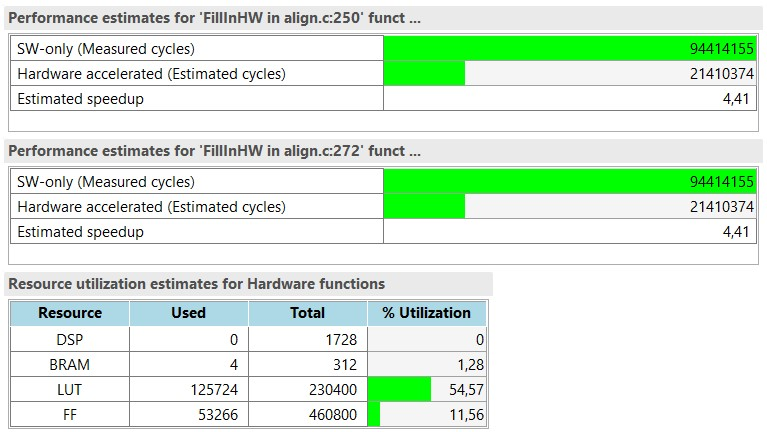
\includegraphics[width=0.8\textwidth]{speedup/speedup.jpg}
	\caption{Latency analyzer in SDSoC. We can see the number of clock cycles spent in the software and the hardware variant of the implementation, as well as the speedup. The speedup is calculated 2 times, since we run the fillIn function twice, once for the forward and once for the reverse sequence. The resource utilization of the FPGA hardware is also visible in this picture}
	\label{fig:speedup}
\end{figure}